\section{Discussion}
\label{sec:discussion}
We will now reason about our proposed techniques and their evaluation by
discussing our operational experience (\S~\ref{sec:operational}), presenting the
balance between transparency and secrecy (\S~\ref{sec:secrecy}), reiterating
our work's shortcomings (\S~\ref{sec:limitations}), and outline the rold cloud
providers play in Sybil attacks (\S~\ref{sec:cloud}).

\subsection{Operational experience}
\label{sec:operational}

\mynote{Mention since when we are running our systems and what it was like.}

\mynote{Difficult to get relays blacklisted because of overloaded dirauth
operators.}

\mynote{Root cause analysis difficult.  Especially if relays behave exactly like
benign relays would.  Weighing up up pros vs. cons when considering to reject a
relay is necessary.}

\subsection{Balancing transparency and secrecy}
\label{sec:secrecy}
During the development of sybilhunter, we pondered what a reasonable balance
between transparency and secrecy could look like.  On the one hand, we want our
system design to be open to stimulate scientific progress.  On the other hand,
a freely available implementation helps attackers evade the system because they
can first test their attacks in an offline setting.

It seems difficult to achieve a setting analogous to Kerckhoffs' principle in
cryptography, which states that a system has to be secure even if all about it
is known---except the key.  There is no key in our setting.  We can, however,
divide our system into the \emph{open} analysis framework and its \emph{secret}
parameters.  It is the analysis framework that is of primary interest to other
researchers, whereas its precise parameters are a mere operational details.

Note that the authors of exitmap follow a similar philosophy by making
available exitmap's scanning framework~\cite{exitmap}, but sharing its
(typically straightforward) modules only privately.  This differentiation seems
to work well as attackers are only interested in scanning modules, e.g., which
URLs, protocols, and ports are probed.

\subsection{Limitations}
\label{sec:limitations}
We mentioned in Section~\ref{sec:threat_model} that we are unable to prevent
all Sybil attacks.  An adversary unconstrained by time and money will always
be able to inject Sybils.  This is already known since Douceur showed in 2002
that the only way to prevent Sybil attacks is a central authority that verifies
network participants~\cite{Douceur2002a}.  A central authority is unlikely to
be viable for the Tor network.  It would be in conflict with Tor's goal of
distributing trust and alienate relay operators.

% We will now explore how costly a Sybil attack is in practice.  First, an
% adversary needs a number of systems to run Tor relays on.  These systems should
% be geographically distributed to maximize IP address diversity.  One option is
% to rent virtual private systems, starting at around \$3 per month for 1 Gbps.
% In 2011, the price for 1,000 compromised systems to install malware on (so
% called \emph{loads}) ranged from \$13 (in Asia) to \$125 (in the U.S.)\cite[\S
% 5]{Stone-Gross2011a}.

\mynote{Try to give a rough estimate of how costly a Sybil attack is.}

\subsection{Use and abuse of cloud providers}
\label{sec:cloud}
Table~\ref{tab:sybils} contains several cloud-hosted Sybil clusters.
Presumably, cloud-hosted relays are attractive to attackers because they
provide cheap, disposable, and hourly-billed platforms.  But does the bandwidth
contributed by cloud-hosted relays make up for the abuse?  We will now discuss
this question.

First, we calculated the amount of bandwidth contributed by Tor relays that
were located in the netblocks of three major cloud providers, Amazon
AWS~\cite{amazonaws}, Google Cloud Platform~\cite{googlecloud}, and Microsoft
Azure~\cite{azure}.  Note that the netblocks published by these cloud providers
can change over time, and are not archived.  As a result, we could have missed
netblocks, which means that our calculations can only provide a \emph{lower
bound} of cloud-hosted bandwidth.

Since we do not have access to archived netblocks, we limit our analysis to
July 2015.  Having obtained cloud-hosted netblocks, we then iterated over all
744 consensus files from July 2015 and identified Tor relays that were hosted
by Google, Amazon, or Microsoft.  On average, 189 out of 6,540 Tor relays
(2.9\%) were run in cloud-powered IP address space.  Because Tor
clients select relays in their circuits based on bandwidth, we then determined
the fraction these cloud-hosted relays contributed to the total Tor bandwidth.
The results are shown in Table~\ref{tab:bwfraction}.  The median contributed
bandwidth is 0.8\%.  There were no Google-hosted relays.  Amazon-hosted relays
contributed about 18 times more bandwidth than Microsoft-hosted relays.

\begin{table}[t]
	\centering
	% \begin{tabular}{lllllll}
	\begin{tabular}{lllll}
	% Provider & Min. & 1st Qu. & Median & Mean & 3rd Qu. & Max. \\
	\textbf{Provider} & \textbf{Min.} & \textbf{Median} & \textbf{Mean} & \textbf{Max.} \\
	\hline
	% Google & 0 & 0 & 0 & 0 & 0 & 0 \\
	Google & 0 & 0 & 0 & 0 \\
	% Amazon & 0.2 & 0.7 & 0.7 & 0.76 & 0.8 & 1.5 \\
	Amazon & 0.2 & 0.7 & 0.76 & 1.5 \\
	% Microsoft & 0 & 0 & 0 & 0.02 & 0 & 0.1 \\
	Microsoft & 0 & 0 & 0.02 & 0.1 \\
	\hline
	% Total & 0.2 & 0.7 & 0.8 & 0.79 & 0.8 & 1.5 \\
	Total & 0.2 & 0.8 & 0.79 & 1.5 \\
	\end{tabular}
	\caption{Percentage of total Tor bandwidth in July 2015 contributed by
	relays hosted in Google's, Amazon's, or Microsoft's cloud.}
	\label{tab:bwfraction}
\end{table}

In addition to Tor relays, there are bridges, which are unpublished Tor relays
that are used for censorship circumvention.  The IP addresses of bridges are
not published, which prevents us from doing the same kind of bandwidth
analysis.  The Tor Project, however, publishes the number of bridges that were
set up using Tor Cloud~\cite{torcloud}, a service to easily set up an
EC2-powered bridge, exploiting Amazon's free usage tier.  The number of Tor
Cloud bridges, illustrated in Figure~\ref{fig:cloudbridges}, can serve as proxy
variable for the amount of bandwidth they contribute.  The number has been
decreasing over time, and on May 8, 2015, the Tor Cloud program was shut down.
As a result, we expect the number of cloud bridges to keep decreasing, as the
free usage tier of more bridge operators runs out.

\begin{figure}[t]
	\centering
	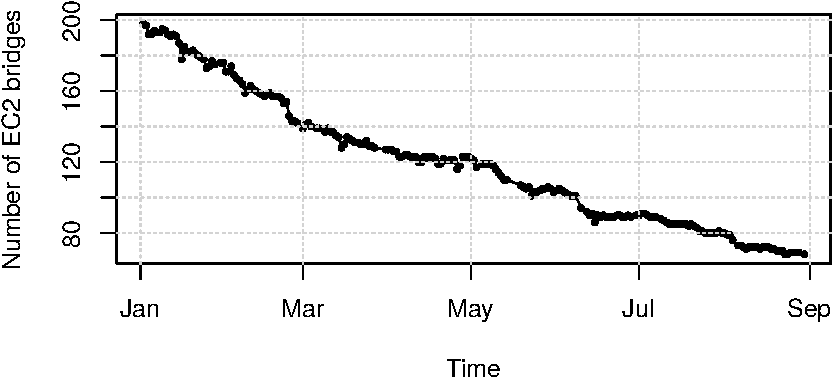
\includegraphics[width=0.48\textwidth]{diagrams/torcloud.pdf}
	\caption{The amount of TorCloud~\cite{torcloud} bridges over time.  The
	numbers are decreasing and the TorCloud system has ended in May 2015.}
	\label{fig:cloudbridges}
\end{figure}
